\savegeometry{fhsststandard}
\newgeometry{paper=a4paper, lmargin=0.1\paperwidth, rmargin=0.1\paperwidth, tmargin=1in, bmargin=1in}


\begin{titlepage}
\begin{adjustwidth}{1in}{1in}
\begin{center}
    \thispagestyle{empty}

    \vspace*{4in}

    {\normalfont\sffamily\fontsize{36}\normalfont\itshape{Everything Maths } \\ \vspace*{1cm}
    {\normalfont\sffamily\fontsize{22}\normalfont\itshape{Graad 10 Wiskunde}}
    \vspace*{1in} \\
    \LARGE Weergawe 1 -- CAPS  \\

   {\vspace*{2in}
     deur Siyavula en vrywilligers 
  

\vfill

    }}
\end{center}
\end{adjustwidth}
\end{titlepage}






% Copyright notice
\newpage
\thispagestyle{empty}
{
\begin{center}
\normalfont\sffamily\fontsize{22}\normalfont\itshape  Kopiereg kennisgewing\\

\vspace*{1in}

\textbf{Jou wetlike vryheid om hierdie boek te kopieer}\\

\end{center}
}

{\large
Jy mag enige gedeelte van hierdie boek vrylik kopieer, trouens ons moedig jou aan om dit doen. Jy kan dit soveel keer as jy wil fotostateer, uitdruk of versprei. Jy kan dit op jou selfoon, iPad, rekenaar of geheue stokkie aflaai. Jy kan dit selfs op ‘n kompakskyf (CD) brand of dit vir iemand per e-pos aanstuur of op jou eie webblad laai.
Die enigste voorbehoud is dat jy die boek, sy omslag en die kortkodes onveranderd laat. \par

Vir meer inligting oor die Creative Commons Attribution-NoDerivs 3.0 Unported (CC BY-ND
3.0) lisensie besoek http://creativecommons.org/licenses/by-nd/3.0/}\\


\vspace*{4in}

\begin{center}
\begin{minipage}{0.6\textwidth}

\includegraphics[width=0.8\textwidth]{title_images/cc2.png}
\end{minipage}
\begin{minipage}{0.3\textwidth}

\includegraphics[width=0.8\textwidth]{title_images/cc1.png}
\end{minipage}
\end{center}

% Authors
\newpage
\thispagestyle{empty}


\begin{flushleft} \textbf{\LARGE  Lys van skrywers} \end{flushleft}

{Hierdie boek is gegrond op die oorspronklike Free High School Science Text wat in sy geheel deur vrywilligers van die akademici, onderwysers en industrie deskundiges geskryf is. Hulle visie was ‘n stel wiskunde en fisiese wetenskappe handboeke, op die kurrikulum gebaseer, wat vrylik aan enige iemand beskikbaar is en onder ‘n oop kopiereg lisensie handel.} \par

\textbf{\large Siyavula kern span} \\

Neels van der Westhuizen; Alison Jenkin; Leonard Gumani Mudau; Marina van Zyl; Helen Robertson; Carl Scheffler; Nicola du Toit; Josephine Mamaroke Phatlane; William Buthane Chauke; Thomas Masango \par

\textbf{\large Oorspronklike Free High School Science Texts kern span}\\

Mark Horner; Samuel Halliday; Sarah Blyth; Rory Adams; Spencer Wheaton \par 


\textbf{\large Oorspronklike Free High School Science Texts redaksie}\\

Jaynie Padayachee; Joanne Boulle; Diana Mulcahy; Annette Nell; René Toerien; Donovan Whitfield \par

\textbf{\large Siyavula en Free High School Science Texts bydraers}\\

    Sarah Abel;
Dr. Rory Adams;
    Andrea Africa;
    Matthew Amundsen;
    Ben Anhalt;
    Prashant Arora;
    Amos Baloyi;
    Bongani Baloyi;
    Raymond Barbour;
    Caro-Joy Barendse;
    Richard Baxter;
    Tara Beckerling;
    Tim van Beek;
    Jennifer de Beyer;
Dr. Sarah Blyth;
    Sebastian Bodenstein;
    Martin Bongers;
    Gareth Boxall;
    Stephan Brandt;
    Hannes Breytenbach;
    Alex Briell;
    Wilbur Britz;
    Graeme Broster;
    Craig Brown;
    Deanne de Bude;
    Richard Burge;
    Bianca Böhmer;
    George Calder-Potts;
    Eleanor Cameron;
    Richard Case;
    Sithembile Cele;
    Alice Chang;
    Richard Cheng;
    Fanny Cherblanc;
Dr. Christine Chung;
    Brett Cocks;
    Stefaan Conradie;
    Rocco Coppejans;
    Tim Craib;
    Andrew Craig;
    Tim Crombie;
    Dan Crytser;
Dr. Anne Dabrowski;
    Laura Daniels;
    Gareth Davies;
    Sean Dobbs;
    Buhle Donga;
    William Donkin;
    Esmi Dreyer;
    Matthew Duddy;
    Fernando Durrell;
Dr. Dan Dwyer;
    Frans van Eeden;
    Alex Ellis;
    Tom Ellis;
    Andrew Fisher;
    Giovanni Franzoni;
    Ingrid von Glehn;
    Tamara von Glehn;
    Lindsay Glesener;
    Kevin Godby;
Dr. Vanessa Godfrey;
    Terence Goldberg;
Dr. Johan Gonzalez;
    Saaligha Gool;
    Hemant Gopal;
Dr. Stephanie Gould;
    Umeshree Govender;
    Heather Gray;
    Lynn Greeff;
    Carine Grobbelaar;
Dr. Tom Gutierrez;
    Brooke Haag;
    Kate Hadley;
    Alex Hall;
Dr. Sam Halliday;
    Asheena Hanuman;
Dr. Melanie Dymond Harper;
Dr. Nicholas Harrison;
    Neil Hart;
    Nicholas Hatcher;
    Jason Hayden;
    Laura Hayward;
Dr. William P. Heal;
    Pierre van Heerden;
Dr. Fritha Hennessy;
    Shaun Hewitson;
    Millie Hilgart;
    Grant Hillebrand;
    Nick Hobbs;
    Chris Holdsworth;
Dr. Benne Holwerda;
Dr. Mark Horner;
    Robert Hovden;
    Mfandaidza Hove;
    Jennifer Hsieh;
    Laura Huss;
    Rowan Jelley;
    Grant Jelley;
    Clare Johnson;
    Luke Jordan;
    Tana Joseph;
Dr. Fabian Jutz;
    Brian Kamanzi;
Dr. Lutz Kampmann;
    Simon Katende;
    Natalia Kavalenia;
    Nothando Khumalo;
    Paul Kim;
Dr. Jennifer Klay;
    Lara Kruger;
    Sihle Kubheka;
    Andrew Kubik;
Dr. Jannie Leach;
    Nkoana Lebaka;
Dr. Marco van Leeuwen;
Dr. Tom Leinster;
    Henry Liu;
    Christopher Loetscher;
    Mike Loseby;
    Amandla Mabona;
    Malothe Mabutho;
    Stuart Macdonald;
Dr. Anton Machacek;
    Tshepo Madisha;
    Batsirai Magunje;
Dr. Komal Maheshwari;
    Michael Malahe;
    Masoabi Malunga;
    Kosma von Maltitz;
    Masilo Mapaila;
    Bryony Martin;
    Nicole Masureik;
    John Mathew;
Dr. Will Matthews;
    Chiedza Matuso;
    JoEllen McBride;
    Nikolai Meures;
    Riana Meyer;
    Filippo Miatto;
    Jenny Miller;
    Abdul Mirza;
    Mapholo Modise;
    Carla Moerdyk;
    Tshwarelo Mohlala;
    Relebohile Molaoa;
    Marasi Monyau;
    Asogan Moodaly;
    Jothi Moodley;
    Robert Moon;
    Calvin Moore;
    Bhavani Morarjee;
    Kholofelo Moyaba;
    Nina Gitau Muchunu;
    Kate Murphy;
    Emmanuel Musonza;
    Tom Mutabazi;
    David Myburgh;
    Kamie Naidu;
    Nolene Naidu;
    Gokul Nair;
    Vafa Naraghi;
    Bridget Nash;
    Tyrone Negus;
    Huw Newton-Hill;
    Buntu Ngcebetsha;
Dr. Markus Oldenburg;
    Thomas O’Donnell;
Dr. Jaynie Padayachee;
    Poveshen Padayachee;
    Masimba Paradza;
    Dave Pawson;
    Justin Pead;
    Nicolette Pekeur;
    Sirika Pillay;
    Jacques Plaut;
    Barry Povey;
    Andrea Prinsloo;
    Joseph Raimondo;
    Sanya Rajani;
Prof. Sergey Rakityansky;
    Alastair Ramlakan;
Dr. Matina J. Rassias;
Dr. Jocelyn Read;
    Jonathan Reader;
    Jane Reddick;
Dr. Matthew Reece;
    Razvan Remsing;
    Laura Richter;
    Max Richter;
    Sean Riddle;
Dr. David Roberts;
    Christopher Roberts;
    Helen Robertson;
    Evan Robinson;
    Raoul Rontsch;
Dr. Andrew Rose;
    Katie Ross;
    Jeanne-Marié Roux;
    Mark Roux;
    Bianca Ruddy;
    Nitin Rughoonauth;
    Katie Russell;
    Steven Sam;
Dr. Carl Scheffler;
    Cho Hee Shrader;
    Nathaniel Schwartz;
    Duncan Scott;
    Helen Seals;
    Relebohile Sefako;
    Sandra Serumaga-Zake;
    Paul Shangase;
    Cameron Sharp;
    Ian Sherratt;
Dr. James Short;
    Roger Sieloff;
    Brandon Sim;
    Bonga Skozana;
    Clare Slotow;
    Bradley Smith;
    Greg Solomon;
    Nicholas Spaull;
Dr. Andrew Stacey;
Dr. Jim Stasheff;
    Mike Stay;
    Mike Stringer;
    Masixole Swartbooi;
    Tshenolo Tau;
    Tim Teatro;
    Ben Thompson;
    Shen Tian;
    Xolani Timbile;
    Nicola du Toit;
    Robert Torregrosa;
    Jimmy Tseng;
    Pieter Vergeer;
    Rizmari Versfeld;
    Mfundo Vezi;
    Mpilonhle Vilakazi;
    Mia de Vos;
    Helen Waugh;
    Leandra Webb;
Dr. Dawn Webber;
    Michelle Wen;
    Neels van der Westhuizen;
Dr. Alexander Wetzler;
Dr. Spencer Wheaton;
    Vivian White;
Dr. Gerald Wigger;
    Harry Wiggins;
    Heather Williams;
    Wendy Williams;
    Julie Wilson;
    Timothy Wilson;
    Andrew Wood;
    Emma Wormauld;
Dr. Sahal Yacoob;
    Jean Youssef;
    Ewald Zietsman;;
Johan Zietsman;
    Marina van Zyl







% Everything Maths page
\newpage
\thispagestyle{empty}

{\normalfont\sffamily\fontsize{22}\normalfont\itshape Everything Maths} \par

{
Ons dink oor die algemeen aan Wiskunde as ‘n vak oor getalle, maar eintlik is Wiskunde ‘n taal. As ons dié taal leer praat en verstaan kan ons baie van die natuur se geheime ontdek. Net soos ons iemand se taal moet verstaan om meer van hom/haar te leer, moet ons wiskunde gebruik om meer te leer van alle aspekte van die wêreld – of dit nou fisiese wetenskappe, lewenswetenskappe of selfs finansies of ekonomie is. \par

Die vernaamste skrywers en digters het ‘n gawe om woorde só te gebruik dat hulle mooi en inspirerende stories kan vertel. Net so kan ons wiskunde gebruik om konsepte te verduidelik en nuwe dinge te skep. Baie van die moderne tegnologie wat ons lewens beter en makliker maak, is afhanklik van wiskunde. DVDs, Google soektogte en bankkaarte wat met ‘n PIN werk, is maar net ‘n paar voorbeelde. Woorde het nie ontstaan om stories te vertel nie, maar die bestaan daarvan maak dit moontlik. Net so is die wiskunde wat gebruik is om hierdie tegnologie te ontwikkel, nie spesifiek vir hierdie doel ontwikkel nie. Die uitvinders kon egter bestaande wiskundige beginsels gebruik wanner en waar die toepassing daarvan nodig was. \par


Trouens is daar nie ‘n enkele faset van die lewe wat nie deur wiskunde geraak word nie. Baie van die mees gesogte beroepe is afhanklik van wiskunde. Siviele ingenieurs gebruik wiskunde om te bepaal hoe om die beste, nuwe ontwerpe te maak. Ekonome gebruik wiskunde om te beskryf en voorspel hoe die ekonomie sal reageer op sekere veranderinge. Beleggers gebruik wiskunde om die prys van sekere soorte aandele te bepaal of om die risiko verbonde aan sekere beleggings te bereken. Wanneer sagteware-ontwikkelaars programme soos Google skryf, gebruik hulle baie van die wiskundige algoritmes om die programme bruikbaar maak.\par

Selfs in ons daaglikse lewens is wiskunde oral – in die afstand wat ons aflê, tyd en geld. Ons kan ook in kuns, ontwerp en musiek die invloed van wiskunde sien, veral in die proporsies en musikale klanke. Hoe beter ons vermoë om wiskunde te verstaan, hoe beter ons vermoë om die natuur en die skoonheid daarvan te waardeer. Wiskunde is daarom nie net ‘n abstrakte dissipline nie, dit omarm logika, simmetrie, harmonie en tegnologiese vooruitgang. Meer as enige ander taal is wiskunde oral en universeel in sy toepassing. \par

Kyk na die video inleiding van Dr. Mark Horner: \raisebox{-0.2em}{
\includegraphics[height=1em]{../icons/video.pdf}} VMiwd by www.everythingmaths.co.za

}





% Webbook page

\newpage
\thispagestyle{empty}

{\normalfont\sffamily\fontsize{22}\normalfont\itshape Meer as net 'n handboek} \par

\begin{center}
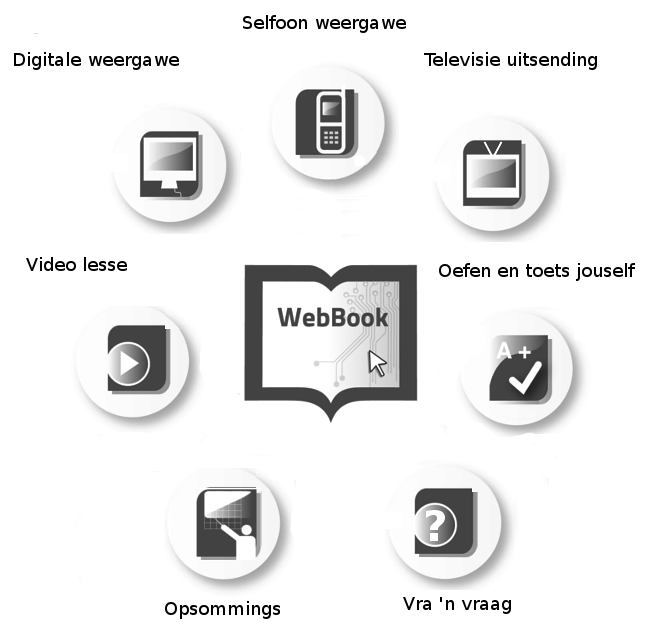
\includegraphics[width=0.70\textwidth]{title_images/morethantextbookAfrikaans.png}
\end{center}

\par
{
\textbf{Everythings Maths} is nie net ‘n Wiskunde handboek nie. Daar is meer in as net die gewone inhoud wat jy van ‘n skoolhandboek verwag. Om mee te begin kan jy die boek aflaai of aanlyn lees op jou selfoon, rekenaar of iPad. Dit is daarom gerieflik beskikbaar waar ook al jy is.\par

Ons weet dat dit partykeer moeilik is om iets in woorde te verduidelik, daarom is daar lesse en verduidelikings in video-formaat by elke hoofstuk sodat die idees en konsepte vir jou realiteit kan word. Die aanbieding aan die einde van elke hoofstuk bied ‘n oorsig oor al die inhoud wat jy geleer het, en die kern konsepte is vir jou uitgelig sodat jy die maklik kan hersien. \par

Al die oefeninge in die boek het ‘n skakel na ‘n diens wat vir jou nog oefeninge gee, die oplossings gee of jou toelaat om jou vaardigheid te toets – op ‘n selfoon of ‘n rekenaar. \par

Ons wil weet wat jy dink, waaroor jy wonder, en waarmee jy sukkel terwyl jy deur die boek werk en die oefeninge probeer doen. Ons het dit daarom moontlik gemaak dat jy jou werk, met jou selfoon of rekenaar, digitaal kan “aansteek” op ‘n bladsy en dan ook te kan sien watter vrae en antwoorde ander lesers “aangesteek” het. \par



}




% mobile or PC
\newpage
\thispagestyle{empty}

{\normalfont\sffamily\fontsize{22}\normalfont\itshape Everything Maths op jou selfoon of rekenaar} \par

{
Jy het altyd toegang tot die handboek, of jy by die huis, die skool of op ‘n trein is. Blaai deur na die aanlyn weergawe van Everything Maths op jou selfoon, “tablet” of rekenaar. As jy dit wil lees terwyl jy van lyn af is, kan jy dit as ‘n PDF-leêr of in e-boek formaat aflaai.\par


Om die boek te lees of af te laai, besoek \textbf{www.everythingmaths.co.za} op jou selfoon of rekenaar.} \vspace*{2cm}

\begin{center}
\begin{minipage}{0.4\textwidth}
\centering
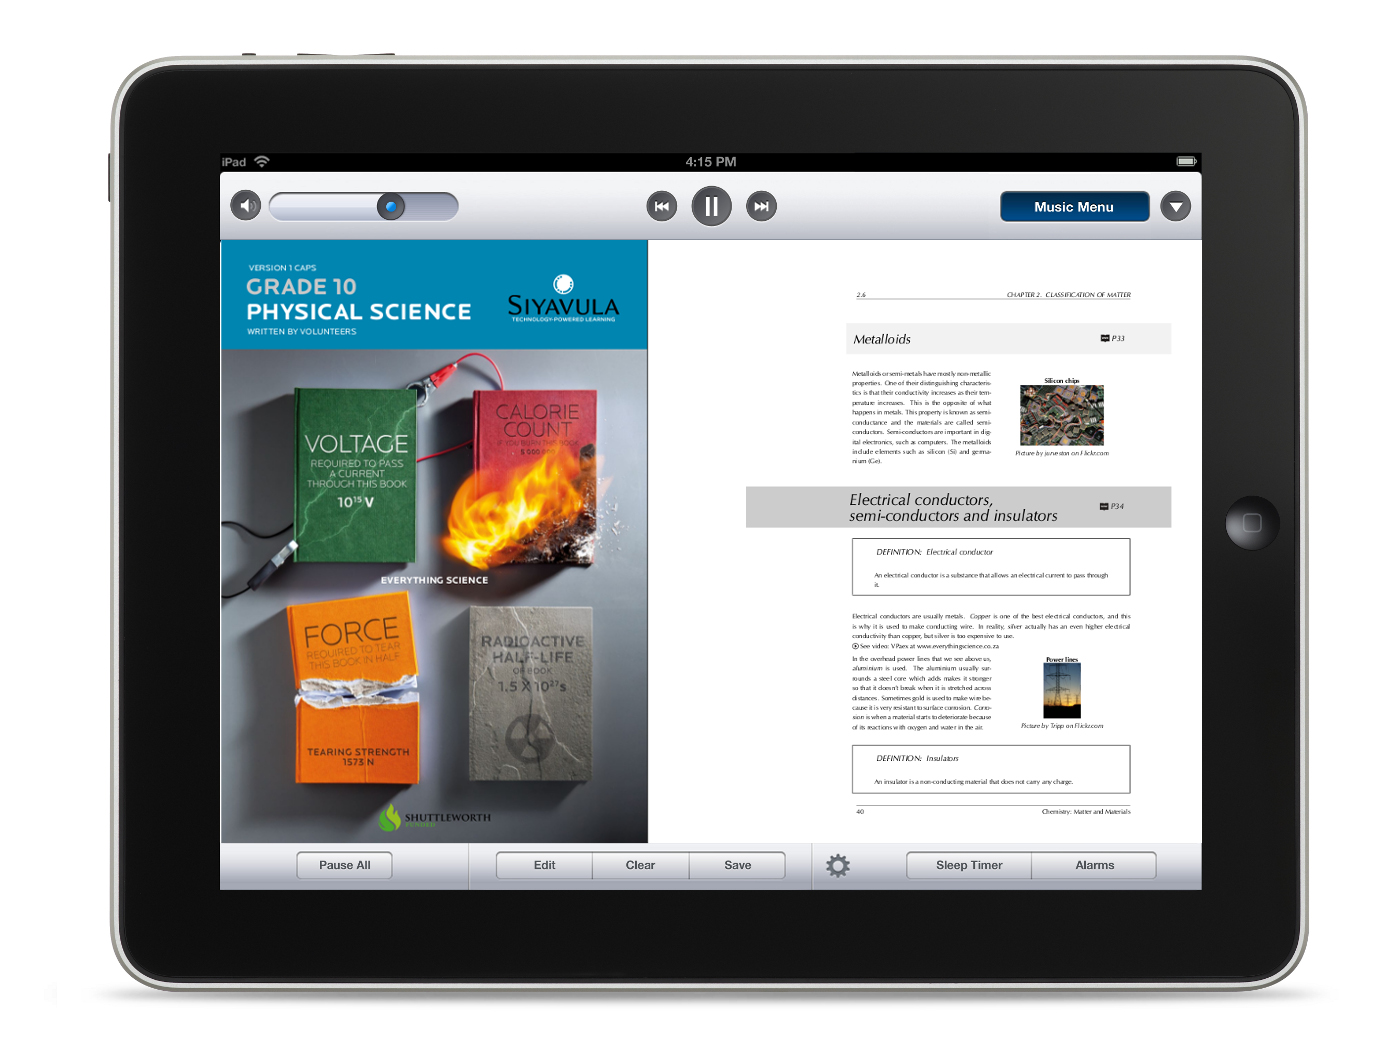
\includegraphics[width=0.8\textwidth]{title_images/ipad.jpg}
\end{minipage}
\begin{minipage}{0.4\textwidth}
\centering
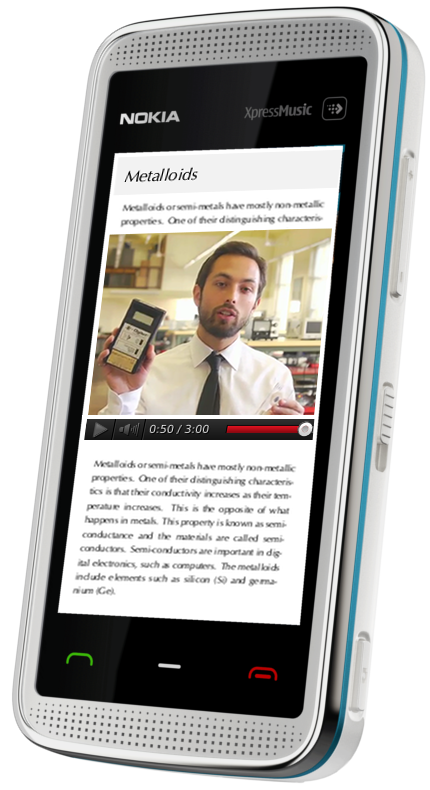
\includegraphics[width=0.4\textwidth]{title_images/phone.png}
\end{minipage}
\end{center}

\vspace*{2cm}


{\normalfont\sffamily\fontsize{22}\normalfont\itshape Gebruik die ikons en kortkodes} \par

{
Die ikons in die boek help jou om te sien waar videos, aanbiedinge, oefeninge en ander hulp voorkom. Die kortkodes langs die ikons laat jou toe om direk na die aanlyn-bron te blaai sonder om daarvoor te soek.\par


\begin{tabular}{lcl}
\raisebox{-0.8em}{
\includegraphics[width=0.8cm]{../icons/www.pdf}} & (A123) & Gaan direk na 'n afdeling\\
\raisebox{-0.8em}{
\includegraphics[width=0.8cm]{../icons/video.pdf}} & (V123) & Video, simulasie of aanbieding \\
\raisebox{-0.8em}{
\includegraphics[width=0.8cm]{../icons/aplus.pdf}} & (P123) & Oefen en toets jou vaardighede \\
\raisebox{-0.8em}{
\includegraphics[width=0.8cm]{../icons/help.pdf}} & (Q123) & Vra vir hulp of vind 'n antwoord \\
\end{tabular}
\par
\vspace*{1cm}

Om die videos aanlyn te sien, oefeninge te doen of ‘n vraag op te sit, gaan na die Everything Maths webblad by \underline{www.everythingsmaths.co.za} van jou selfoon of rekenaar en voer die kortkode in die soek-blokkie in.
}




% video lessons
\newpage
\thispagestyle{empty}

{\normalfont\sffamily\fontsize{22}\normalfont\itshape Video-lesse} \par

{

Soek die video ikons in die boek. Hierdie ikons neem jou na video-lesse wat sal help om die idees en konsepte vir jou lewendig te maak. Jy kan ekstra insigte, volledige verduidelikings en uitgewerkte voorbeelde hier sien. Die konsep word prakties voorgestel en jy kan luister hoe regte mense wiskunde en wetenskap in hul werk gebruik. \par

\begin{figure}[h]
\begin{center}
Sien video verduideliking \raisebox{-0.6em}{
\includegraphics[width=0.7cm]{../icons/video.pdf}} (Video: V123)\\
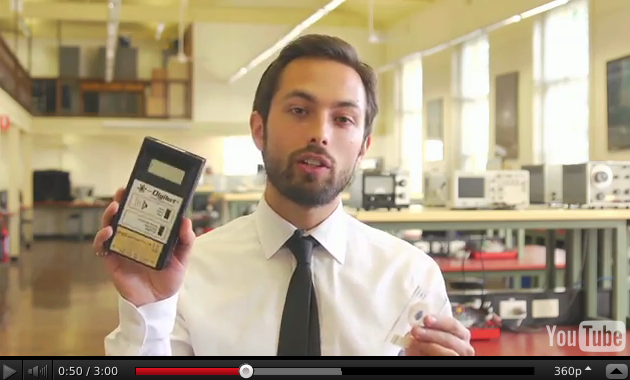
\includegraphics[width=0.5\textwidth]{title_images/veritasiumvideo.png}
\end{center}
\end{figure}

}
{\normalfont\sffamily\fontsize{22}\normalfont\itshape Video oefeninge} \par

{

As daar oefeninge in die boek is, sal jy die ikons en kortkodes vir video-oplossings, oefeninge en hulp sien. Hierdie kortkodes vat jou na die video-oplossings van sommige oefeninge sodat jy stap-vir-stap kan sien hoe om die probleem op te los. \par

\begin{figure}[h]
\begin{center}
Sien video oefening \raisebox{-0.6em}{
\includegraphics[width=0.7cm]{../icons/video.pdf}} (Video: V123)\\ 
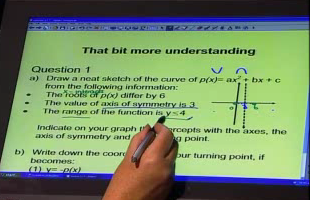
\includegraphics[width=0.5\textwidth]{title_images/mindsetexercise.png}
\end{center}
\end{figure}
Jy kan toegang tot die videos kry deur:
\begin{itemize}
\item hulle aanlyn op jou selfoon of rekenaar te kyk
\item die videos af te laai sodat jy die van lyn af op jou selfoon of rekenaar kan kyk.
\item ‘n DVD te bestel wat jy op jou TV of rekenaar kan speel.
\item dit van lyn af af te laai met Bluetooth of Wi-Fi van sekere afsetpunte
\end{itemize}
}


% practise and test your skills
\newpage
\thispagestyle{empty}
{

Om nog videos te sien, of vir meer inligting, besoek die Everything Maths webblad vanaf jou selfoon of rekenaar by \underline{www.everythingmaths.co.za}  
\vspace*{1cm}
\\
{\normalfont\sffamily\fontsize{22}\normalfont\itshape Oefen en toets jou vaardigheid} \par


Een van die beste maniere om vir toetse of eksamens voor te berei, is om te oefen om dieselfde soort vrae te antwoord as waarmee jy getoets gaan word. By elke stel oefeninge is daar ‘n oefen ikon en ‘n kortkode. Hierdie aanlyn-oefeninge, wat jy van jou selfoon of rekenaar af lan laai, hou rekord van jou prestasie en vordering, gee vir jou terugvoer oor watter areas jy mee sukkel en maak voorstelle oor na watter afdelings of videos jy moet gaan kyk.


\begin{figure}[h]
\begin{center}
Sien meer oefeninge  \raisebox{-0.6em}{
\includegraphics[width=0.7cm]{../icons/aplus.pdf}} (QM123)\\ 
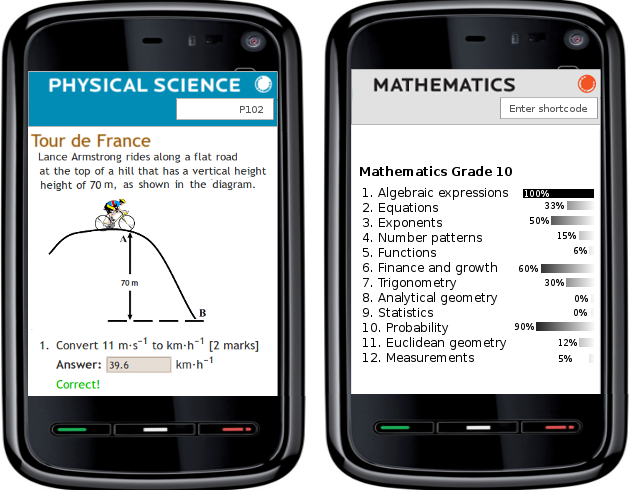
\includegraphics[width=0.65\textwidth]{title_images/practicephones.png}
\end{center}
\end{figure}
\par


Om te oefen en jou vaardigheid te toets:\par

Gaan na \underline{www.everythingmaths.co.za} op jou selfoon of rekenaar en voer die kortkode in.\partykeer
\vspace*{1cm}

%{\normalfont\sffamily\fontsize{22}\normalfont\itshape Television broadcasts} \par
%This book is the same one used by \textbf{Mindset Learn} in their television broadcast where experienced
%educators explain the key concepts, perform live experiments and work out exercises from the book.
%\textbf{Mindset Learn} broadcasts a full 28 hours of curriculum support each week of term. \par
%
%
%Maths can be seen on Mondays and Science on Tuesdays. There is also Life Sciences on Wednesdays
%and Maths Literacy on Thursdays. Revision of the week's work is done on Saturdays for Grade 12 and on
%Sundays for Grades 10 and 11.


}


\newpage
\thispagestyle{empty}

{\normalfont\sffamily\fontsize{22}\normalfont\itshape Vra vrae en vind antwoorde} \par

{

% Have you ever had a question about a specific fact, formula or exercise in your textbook and wished you could just ask someone? Surely someone else in the country must have had the same question at the same place in the textbook.\par 
Het jy al ooit 'n vraag oor n spesifieke feit, formule of 'n oefening in jou handboek gehad en gewens dat jy net iemand kon vra? Sekerlik moes iemand anders in die land al dieselfde vraag op dieselfde plek in die handboek gehad het.\par

% We invite you to open the textbook on your mobile phone or computer and pin your question at that  exact spot in the textbook using the shortcode. You will be able to see whether it has been asked before and what the given answer to that question is. \par
Ons nooi jou om die handboek op jou selfoon of rekenaar oop te maak en om jou vraag op daardie presiese plek in die handboek op te sit, met die gebruik van die kortkode. Jy sal kan sien of dit al voorheen gevra is en wat die antwoord vir daardie vraag was \par.

% The short codes at section headings helps you navigate to sections in the book to ask and view questions for that section. The short codes for the exercises lets you look at questions and answers relating to those specific exercises.\par
Die kortkodes by afdeling opskrifte help jou om na dele in die boek blaai om vrae te vra en vrae vir daardie afdeling te sien. Die shortcodes vir die oefeninge laat jou kyk na die vrae en antwoorde met betrekking tot daardie spesifieke oefeninge.\par

\begin{tabular}{lcl}
\raisebox{-0.8em}{
\includegraphics[width=0.8cm]{../icons/www.pdf}} & (A123) & Besoek hierdie afdeling om vrae te kyk of te pos\\ %Visit this section to post or view questions
\raisebox{-0.8em}{
\includegraphics[width=0.8cm]{../icons/help.pdf}} & (Q123) &  Vrae of help met 'n spesifieke vraag \\ %Questions or help with a specific question
\end{tabular}



\begin{figure}[h]
\centering
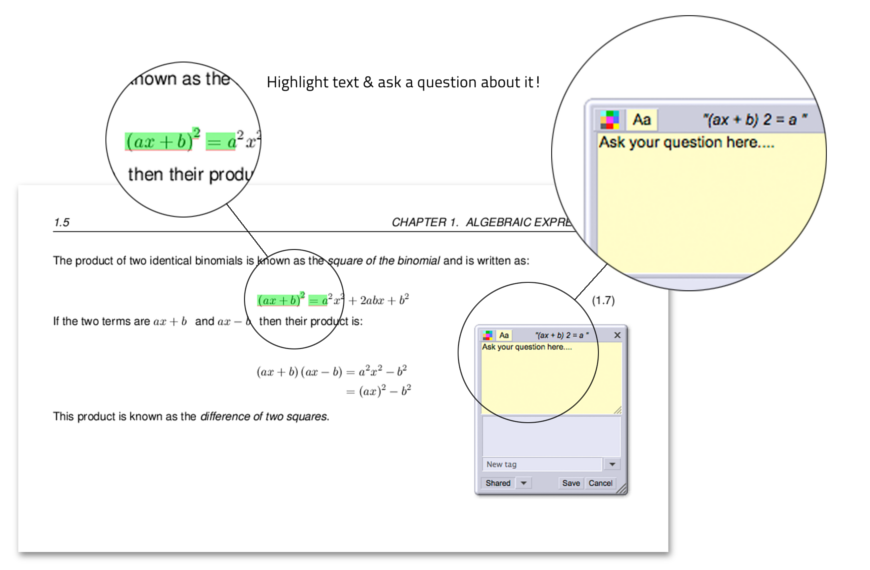
\includegraphics[width=\textwidth]{title_images/questions.png}
\end{figure}


}


%% practise and test your skills
%\newpage
%\thispagestyle{empty}
%{\Large
%
%\begin{table*}[h]
%\large
%\begin{tabular}{lll}
%\textbf{Maths and Science Broadcasts}&&\\
%Grade 10  Maths & Mondays at 4pm & Every second Sunday at 1pm\\
%Grade 11  Maths & Mondays at 5pm & Every second Sunday at 9am\\
%Grade 12  Maths & Mondays at 6pm & Every Saturday at 9am\\
%Grade 10  Science & Tuesdays at 4pm & Every second Sunday at 1pm\\
%Grade 11  Science & Tuesdays at 5pm & Every second Sunday at 9am\\
%Grade 12  Science & Tuesdays at 6pm & Every Saturday at 11am\\
%\textbf{Other broadcasts} & & \\
%Grade 10  Life Science & Wednesdays at 4pm & Every second Sunday at 3pm\\
%Grade 11  Life Science & Wednesdays at 5pm & Every second Sunday at 9am\\
%Grade 12  Life Science & Wednesdays at 6pm & Every Saturday at 1pm\\
%Grade 10  Maths Literacy & Thursdays at 4pm & Every second Sunday at 3pm\\
%Grade 11  Maths Literacy & Thursdays at 5pm & Every second Sunday at 9am\\
%Grade 12  Maths Literacy & Thursdays at 6pm & Every Saturday at 3pm\\
%\end{tabular}
%\end{table*}
%
%
%\textbf{You can watch these live sessions on:}
%\begin{itemize}
%    \item Mindset free-to-air for schools (ask your school)
%    \item Channels 319 on DStv
%    \item Toptv on 319 on TopTV
%\end{itemize}


%}

% Put the margins back for the rest of the book

\loadgeometry{fhsststandard}

\normalfont
